\scanpage{16}
Résumé de quelques résultats de Kostant (sous groupes simples de rang $1$).

$G$ est un groupe semi-simple sur un corps $k$ de car. nulle, $\handwritten{\unsure{\mathfrak{g}|\mathscr{G}}}$ son algèbre de Lie,
% Interlinear handwritten bibliographical note, between the two lines of the definition.
\margin{\handwritten{(The principal 3-dimensional subgroup...., Am. Jour. Oct.1959, 3.4, 3.5, 3.6, 1.2, 9.3)}}

\uline{Théorème} 1. \inserted{\handwritten{(i)}} Soient $x,e\handwritten{\in\mathfrak{g}}$,\inserted{(avec $e\handwritten{\ne}0$, $e$ nilpotent.\,)} Pour tout entier $k$, soit $\handwritten{\mathfrak{g}}(k)$ le sous-espace propre de\hspace{1.5em} correspondant à la valeur propre $k$. Donc si $x=\operatorname{Lie}(i)(1)$, où $i:\underline{G}_m\handwritten{\longrightarrow}G$, les $\handwritten{\mathfrak{g}}(k)$ sont les \deleted{décomposition} composants de $\handwritten{\mathfrak{g}}$ suivant les caractères de $\underline{G}_m$, opérant sur $\handwritten{\mathfrak{g}}$ via $i$ et la représentation adjointe. Les conditions suivantes sont équiva\deleted{\unsure{e}}lentes:

\[
\begin{aligned}
\text{a)}\quad &e\handwritten{\in\mathfrak{g}}(2)\quad\text{i.e.}\quad \handwritten{[}x,e\handwritten{]}=2e,\quad\text{et }\inserted{\text{pour tout entier }k\handwritten{\geq}1,}\\
&\operatorname{ad}(e)^k:\handwritten{\mathfrak{g}}(-k)\handwritten{\longrightarrow\mathfrak{g}}(k)\quad\text{est un }\unsure{\text{isom.}|\text{isom}}
\end{aligned}
\]

\[
\text{b)}\quad e\handwritten{\in\mathfrak{g}}(2),\quad\deleted{\unsure{et}}\quad \operatorname{ad}(e):\handwritten{\mathfrak{g}}(0)\handwritten{\longrightarrow\mathfrak{g}}(-2)\quad\text{est surjectif},
\]
\inserted{\handwritten{et $x$ est de la forme $f(x_{\unsure{o|0}})$, par $f:\operatorname{Sl}(2,\unsure{k'|k})\unsure{\longleftrightarrow|\longrightarrow}G$ (\uline{élément de Dynkin}).}}

\handwritten{\deleted{b') Comme b), avec $\operatorname{ad}(e):\mathfrak{g}(0)\to\mathfrak{g}(\unsure{2|-2})$ \uline{\unsure{bijectif}}}}

\[
\text{c)}\quad e\handwritten{\in\mathfrak{g}}(2),\quad\text{et }x\handwritten{\in}\operatorname{ad}(e)(\handwritten{\mathfrak{g}}).
\]

\[
\text{c')}\quad e\handwritten{\in\mathfrak{g}}(2),\quad\text{et }x\handwritten{\in}\operatorname{ad}(e)(\handwritten{\mathfrak{g}}(-2)).
\]

d) Il existe un homomorphisme $f:\operatorname{Sl}(2,k)\handwritten{\longrightarrow}G$ tel que $f^{\handwritten{'}}(e_o)=e,f^{\handwritten{\unsure{''|'}}}(x_o)=x\deleted{y}$ où $(x_o,e_o,f_o)$ est la base de $\operatorname{Lie}\operatorname{Sl}(2,k)$ correspondant à l'épinglage habituel de ce groupe.

C$\overset{\unsure{-}}{\underset{\text{\unsure{e}}}{\text{e}}}$s conditions impliquent qu'i\deleted{\unsure{o}}l existe un homomorphisme $i:\underline{G}_m\handwritten{\longrightarrow}G$, tel que $\operatorname{Lie}(i)(1)=x$, a fortiori que $x$ est semi-simple. De plus, le $f$ de d) est déterminé de façon unique.

(ii) Pour tout élément nilpotent $e$ de $\handwritten{\mathfrak{g}}$, il existe un \unsure{homomorphisme} $f:\operatorname{Sl}(2,k)\handwritten{\longrightarrow}G$ tel que $f(e_o)=e$, ou ce qui revient au même, tel que $f(u_o)=u$ (où $u=\exp(e)$, $u_o=\exp(e_o)$);\inserted{\handwritten{$f$ est uniquement déterminé \unsure{par} $x=f(x_o)$ i.e., par $i=f\circ i_o$.}} \deleted{e}\handwritten{E}n vertu de (i), il revient au même,\deleted{(}lorsque $e=0$ i\handwritten{/}.e. $u\handwritten{\ne}1$, de dire qu'il existe un $x\handwritten{\in\mathfrak{g}}$ tel que $(x,e)$ satisfasse aux conditions équivalentes de (i), ou encore un homomorphisme $i:\underline{G}_m\handwritten{\longrightarrow}G$ tel que $(\operatorname{Lie}(i)(1),e)$ y satisfasse. Les homomorphismes $f$ en question sont conjugués
% The raised typed par has no caret; its attachment is unresolved. Z= is also raised, farther right.
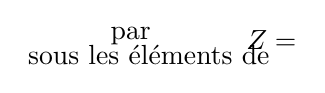
\begin{tikzpicture}[baseline=(cancel.base)]
\node[anchor=base west,inner sep=0] (cancel) at (0,0) {\deleted{sous les éléments de}};
\path (cancel.base west) -- (cancel.base east) coordinate[pos=.34] (parpos) coordinate[pos=.90] (zpos);
\node[anchor=base west,inner sep=0,yshift=2.1ex] at (parpos) {par};
\node[anchor=base west,inner sep=0,yshift=1.3ex] at (zpos) {\handwritten{$Z=$}};
\end{tikzpicture}
$\operatorname{Cent}(e)=\operatorname{Cent}(u)$ (i.e. pour $e\handwritten{\ne}0$, les $x$ en question, ou encore les $i$ en question, sont conjugués \deleted{sous} par $\operatorname{Cent}(u)$), et lorsque $e\handwritten{\ne}0$, les \deleted{\unsure{morphismes}\quad $g$\quad $\operatorname{int}(g)$} $f$ en question (ou encore les
% archive sheet number: 15
